\uuid{q40o}
\exo7id{5819}
\titre{exo7 5819}
\auteur{rouget}
\organisation{exo7}
\datecreate{2010-10-16}
\isIndication{false}
\isCorrection{true}
\chapitre{Conique}
\sousChapitre{Parabole}
\module{Géométrie}
\niveau{L2}
\difficulte{}

\contenu{
\texte{

}
\begin{enumerate}
    \item \question{(Droite de \textsc{Simson}) Soient $ABC$ un triangle et $M$ un point du plan. 

Montrer que les projetés orthogonaux $P$, $Q$ et $R$ du point $M$ sur les côtés $(BC)$, $(CA)$ et $(AB)$ du triangle $ABC$ sont alignés si et seulement si $M$ est sur le cercle circonscrit au triangle $ABC$. La droite passant par les points $P$, $Q$ et $R$ s'appelle la droite de \textsc{Simson} du point $M$ relativement au cercle $(ABC)$.}
\reponse{Soit $M$ un point du plan.

\textbf{1er cas.} Supposons que $M\notin(AB)\cup(AC)\cup(BC)$. 

\begin{align*}\ensuremath
P,\;Q\;\text{et}\;R\;\text{alignés}\Leftrightarrow\left(\overrightarrow{PQ},\overrightarrow{PR}\right)=0\;[\pi]
\Leftrightarrow\left(\overrightarrow{PQ},\overrightarrow{PM}\right)=\left(\overrightarrow{PR},\overrightarrow{PM}\right)\;[\pi].
\end{align*}

Maintenant, puisque les triangles $MPC$ et $MQC$ sont rectangles en $P$ et $Q$ respectivement, les points $P$ et $Q$ sont sur le cercle de diamètre $[MC]$. On en déduit que $\left(\overrightarrow{PQ},\overrightarrow{PM}\right)=\left(\overrightarrow{CQ},\overrightarrow{CM}\right)\;[\pi]$. De même, $\left(\overrightarrow{PR},\overrightarrow{PM}\right)=\left(\overrightarrow{BR},\overrightarrow{BM}\right)\;[\pi]$. Par suite,

\begin{align*}\ensuremath
P,\;Q\;\text{et}\;R\;\text{alignés}&\Leftrightarrow\left(\overrightarrow{CQ},\overrightarrow{CM}\right)=\left(\overrightarrow{BR},\overrightarrow{BM}\right)\;[\pi]\\
 &\Leftrightarrow\left(\overrightarrow{CA},\overrightarrow{CM}\right)=\left(\overrightarrow{BA},\overrightarrow{BM}\right)\;[\pi]\\
 &\Leftrightarrow M\;\text{appartient au cercle circonscrit au triangle}\;ABC\;(\text{privé des points}\;A,\;B\;\text{et}\;C).
\end{align*}

\textbf{2ème cas.} Supposons par exemple que $M\in(AB)$. Dans ce cas, $M=R$. Si de plus $M$ n'est ni $A$, ni $B$, alors $M\neq P$ et $M\neq Q$ puis les droites $(MP)$ et $(MQ)$ sont perpendiculaires aux droites $(BC)$ et $(AC)$ respectivement. Si par l'absurde, les points $P$, $Q$ et $R$ sont alignés, on a $(MP)=(MQ)$ et donc $(AB)//(AC)$. Ceci est une contradiction.

Donc, si les points $P$, $Q$ et $R$ sont alignés, $M$ est l'un des trois points $A$, $B$ ou $C$. La réciproque est immédiate.

En résumant les deux cas,

\begin{center}
\shadowbox{
$P$, $Q$ et $R$ sont alignés si et seulement si $M$ est sur le cercle circonscrit au triangle $ABC$.
}
\end{center}

$$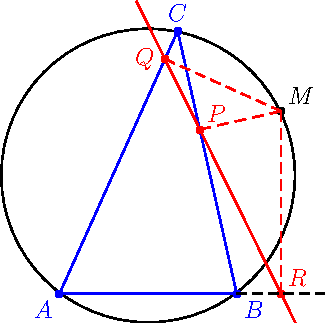
\includegraphics{../images/pdf/q40o-1.pdf}$$}
    \item \question{(Parabole tangente aux trois côtés d'un triangle) Lieu des foyers des paraboles tangentes à trois droites deux à deux non parallèles. Fournir en particulier la construction des points de contacts.}
\reponse{\textbf{Parabole tangente aux trois côtés d'un triangle.} Commençons par rappeler une construction usuelle de la tangente en un point d'une parabole : le triangle $FMH$ est isocèle en $M$ et la tangente en $M$ à $\mathcal{P}$ est la médiatrice du segment $[FH]$. Par suite, le projeté orthogonal $P$ de $F$ sur la tangente $(T)$ est sur $5T_0)$ la tangente au sommet de la parabole $\mathcal{P}$.

$$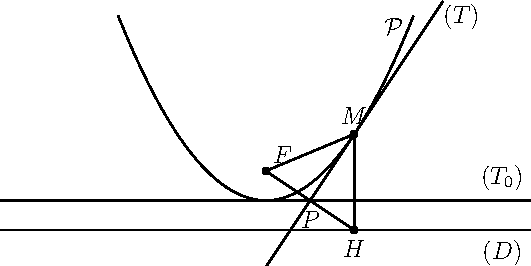
\includegraphics{../images/pdf/q40o-2.pdf}$$



Soient $A$, $B$ et $C$ trois points non alignés. Si $\mathcal{P}$ est une parabole tangente aux droites $(BC)$, $(CA)$ et $(AB)$, les projetés orthogonaux $P$, $Q$ et $R$ de son foyer $F$ sur les droites  $(BC)$, $(CA)$ et $(AB)$ sont alignés sur la tangente au sommet de la parabole $\mathcal{P}$. D'après 1), le point $F$ est nécessairement sur le cercle circonscrit au triangle $ABC$.

Réciproquement, si $F$ est l'un des trois points $A$, $B$ ou $C$, $F$ n'est pas solution car une tangente à une parabole ne passe jamais par son foyer.

Soit donc $F$ un point du cercle circonscrit au triangle $ABC$ et distinct des points $A$, $B$ et $C$. Montrons alors qu'il existe une parabole de foyer $F$, tangente aux droites $(BC)$, $(CA)$ et $(AB)$.

On construit les projetés orthogonaux $P$, $Q$ et $R$ de $F$ sur les droites $(BC)$, $(CA)$ et $(AB)$. Ils sont alignés sur la droite de \textsc{Simson} $(T_0)$ de $F$ relativement au triangle $ABC$. La parabole de foyer $F$ et de tangente au sommet $(T_0)$ est solution du problème posé. La construction des  points de contact est fournie par le graphique de la page précédente : on construit les symétriques de $F$ par rapport aux points $P$, $Q$ et $R$ (ces symétriques sont sur la directrice) puis on remonte perpendiculairement à $(T_0)$ jusqu'à la parabole.

$$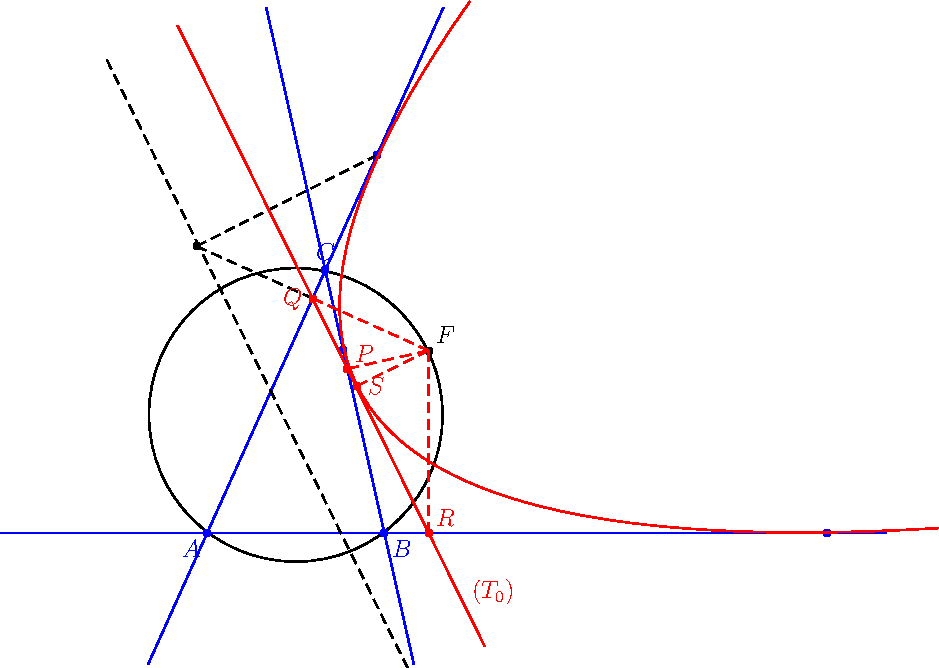
\includegraphics{../images/pdf/q40o-3.pdf}$$}
\end{enumerate}
}
